\documentclass{article}

\usepackage{multirow}
\usepackage{graphicx}
\usepackage{hyperref}
\usepackage{mathtools}

\DeclarePairedDelimiter\ceil{\lceil}{\rceil}
\DeclarePairedDelimiter\floor{\lfloor}{\rfloor}

\title{Homework One}
\date{27 oct 2019}
\author{Iacobescu Tudor, A6}

% preamble stuff for centering every figure
\makeatletter
\g@addto@macro\@floatboxreset\centering
\makeatother

\begin{document}
	\maketitle
	\pagenumbering{arabic}
	
	\section{Introduction}
    \paragraph{}
    The following document details an experiment in which three optimization algorithms are ran against four multi-dimensional functions in order to try and obtain the functions' global minima.
    \paragraph{}
    The purposes of the experiment were initially to compare the three algorithms and how they operate, but it ended up being more interesting for the purposes of highlighting possible problems that pop up when implementing algorithms such as these. These problems don't make the algorithms unusable, but they do complicate their proper implementation.
    \paragraph{}
    The paper will describe the method of the experimental procedure, show the resulting data, and analyze it to try and find some interesting results -- namely, what abnormalities are present in the data and what may have caused them.

	\section{Method}
	\paragraph{}
    For the experiment, we will use two C++ implementations of Iterated Hillclimbing (with a First Ascent and Steepest Ascent approach respectively), as well as an implementation of Simulated Annealing. These algorithms will be tested against four common optimization algorithm testing functions, and their results will be compared.

    \subsection{Algorithm}
    \paragraph{}
    All three of the algorithms rely on representing real numbers from a given interval \([a, b]\) as a string of bits. These bits simulate integers from 0 to \(2^n\) (where n is the number of bits) corresponding roughly to values within the search interval. The number of bits necessary corresponds to the precision (\(10^{-p}\)) wanted:
    $$n = \ceil{\log_2{(b - a) \cdot 10^p}}$$

    \paragraph{}
    A point in d-dimensional space can be represented as a string of \(d \cdot n\) bits. The set of a point's neighbors is that of all the bitstrings of Hamming distance of one from that point's bitstring.
    
    \begin{figure}[!h]
        \centering
        $$00100110$$
        $$10100110, 01100110, 00000110, 00110110$$
        $$00101110, 00100010, 00100100, 00100111$$
        \caption{A point represented by a string of 8 bits, and all of its neighbors.}
    \end{figure}

    \subparagraph{Observation} 
    Assume the above is a point in one-dimensional space. Notice how neighbors whose differing bits are further to the left are farther in space from the original - exponentially farther, in fact. This property makes it so that neighbors end up being more common closer to the point in space than farther away, which effectively makes bigger jumps less likely.

    \paragraph{Iterated Hillclimber}
    This algorithm works by taking a number of randomly placed points in the domain of the function. For each candidate point, we then go through their neighbors to find a better candidate. We stop when we can no longer find a better neighbor. The result of the algorithm is the best point found by any of the chains above -- the point found thus far where the function has the smallest value.
    
    \begin{verbatim}
    function iteratedHillclimber():
        vb = INITIAL_ASSUMED_BEST_CANDIDATE;
        for (i in 0..NUM_ATTEMPTS):
            vc = randomCandidate()
            repeat:
                vn = pickBetterNeighbor(vc)
                if (vc is null):
                    break loop
            if (vc better than vb):
                vn = vc;
        return vb;
    \end{verbatim}

    \paragraph{}
    What separates Iterated Hillclimber into two variants is the way we pick the next neighbor to continue with for each candidate.
    \subparagraph{First ascent} 
    This method iterates through the neighbors only until a better one is found. The candidate is then replaced with said neighbor, and the cycle repeats.
    \begin{verbatim}
    function pickNeighbor(vc): 
        neighbors = generateNeighbors(vc)
        for (vn in neighbors):
            if (vn better than vc)
                return vn
        return null
    \end{verbatim}
    \subparagraph{Steepest ascent}
    This method iterates through all of a candidate's neighbors, and selects the best one (i.e. the one where the function takes the lowest value in) as the one to continue with.
    \begin{verbatim}
    function pickNeighbor(vc):
        neighbors = generateNeighbors(vc)
        vb = neighbors.pickAny()
        for (vn in neighbors):
            if (vn better than vb)
                vb = vn
        if (vb better than vc)
            return vb
        else
            return null
    \end{verbatim}

    \paragraph{Simulated annealing}
    This algorithm shares some similarities with Iterated Hillclimbing. Simulated Annealing takes inspiration from the real life process of annealing -- a heat treatment process where a material such as metal or glass is repeatedly heated and cooled in order to make it more workable. 
    \paragraph{}
    The algorithm works by picking a starting "temperature", and a random starting candidate point. A loop then goes through the candidate's neighbors -- several methods can be used here, but I personally opted for randomly picking one a few times -- and replacing the candidate upon finding a better neighbor. The thing that sets SA apart from Iterated Hillclimbing is the fact that even if a better neighbor is not found, there is still a chance that it might replace the candidate. This allows Simulated Annealing to go uphill as well instead of only downhill, which can allow it to have better odds of finding the global minimum instead of stopping at one of the local minima of the function, like Hillclimbing.
    \paragraph{}
    The chance that a worse neighbor will be picked to continue the algorithm is based on two factors - the difference between the current candidate and the neighbor (the worse the neighbor, the lower the chance) as well as the temperature of the current annealing stage (the higher the temperature, the higher the chance). Once a better neighbor is not found and a worse one fails this check as well, the temperature is lowered, and the cycle repeats until a certain stopping treshhold.

    \paragraph{}
    The following is a simplification of the implementation of Simulated Annealing used for this experiment.

    \begin{verbatim}
    function simulatedAnnealing():
        T = ANNEALING_INITIAL_TEMPERATURE
        t = 0;
        vc = randomCandidate()
        while (T > ANNEALING_STOPPING_TRESHHOLD):
            consecutiveFailures = 0
            while (consecutiveFailures < ANNEALING_CONSEC_FAIL_LIM):
                vn = randomNeighbor(vc)

                if (vn better than vc):
                    vc = vn
                    consecutiveFailures = 0
                else:
                    if (random0to1() < chanceTreshhold(T, vn, vc)):
                        vc = vn
                        consecutiveFailures = 0
                    else:
                        consecutiveFailures++
            T = lowerTemp(T, t)
            t++
        
        return vc

    function chanceTreshhold(T, vn, vc):
        diff = absolute difference between vn and vc's function values
        base = -(diff / T)
        return exp(base)
    
    function lowerTemp(T, t):
        fraction = (t + 1) / (t + 2)
        return T * fraction
    \end{verbatim}
    
	\subsection{Functions}
	The four functions used for this experiment are the Sphere function, the Dixon \& Price function, Michalewicz's function, and Rastrigin's function. The following subsections include the function expression and graph for each of these. The graph is for the two-dimensional version of each function, in its given search interval, with the vertical axis being the value of the function.

	\subsubsection{Sphere function}
	$$f(x_1 \cdots x_n) = {\sum_{i=1}^{n} x_i^{2}}, x_i \in [-5.12, 5.12]$$

	\begin{figure}[!h]
		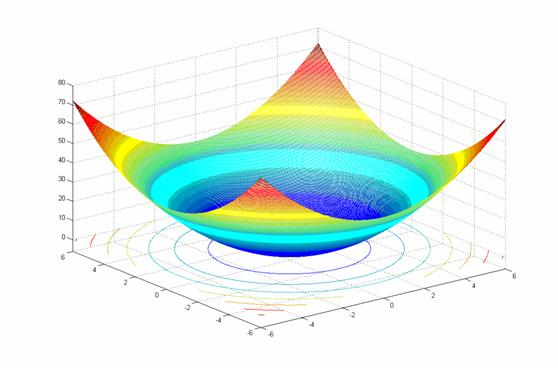
\includegraphics[height=150pt,keepaspectratio]{images/sphere-graph.jpg}
		\caption{Sphere function graph}
	\end{figure}

    
	\subsubsection{Dixon \& Price function}
	$$f(x_1 \cdots x_n) = (x_1 - 1)^2 ) + {\sum_{i=2}^{n} i(2x_i^{2} - x_{i-1})^2}, x_i \in [-10, 10]$$


	\begin{figure}[h]
		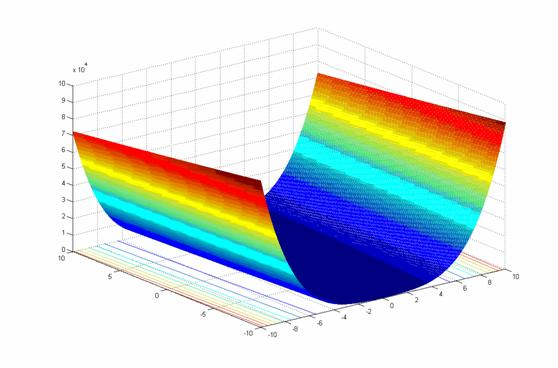
\includegraphics[height=150pt,keepaspectratio]{images/dixon-graph.jpg}
		\caption{Dixon \& Price function graph}
	\end{figure}

	\subsubsection{Michalewicz function}
	$$f(x_1 \cdots x_n) = -{\sum_{i=1}^{n} sin(x_i)\left[\frac{ix_i^2}{\pi}\right]^{2m}}, m = 10, x \in [0, \pi]$$

	\begin{figure}[h]
		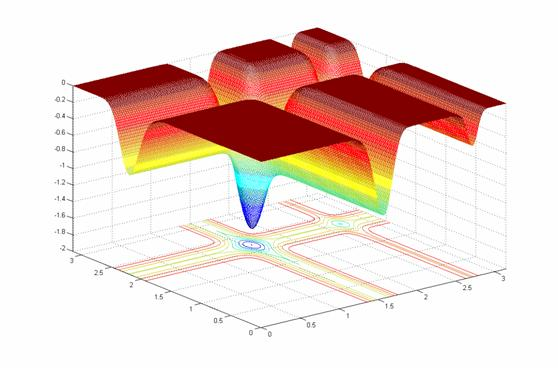
\includegraphics[height=150pt,keepaspectratio]{images/michalewicz-graph.jpg}
		\caption{Michalewicz function graph}
	\end{figure}

	\subsubsection{Rastrigin function}
	$$f(x_1 \cdots x_n) = 10n + \sum_{i=1}^n (x_i^2 -10cos(2\pi x_i)),$$

	\begin{figure}[h]
		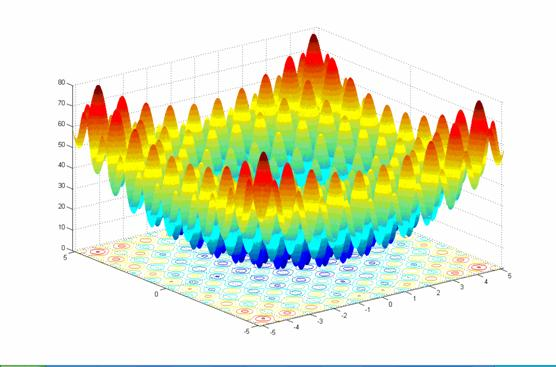
\includegraphics[height=150pt,keepaspectratio]{images/rastrigin-graph.jpg}
		\caption{Rastrigin function graph}
	\end{figure}
	
	\section{Experiment}
	The above algorithms were implemented in C++. For each of the four functions (for 2, 5 and 30 dimensions) all three of the algorithms were ran 30 times in parallel, each run limited to a time just above 600000ms (10 minutes). The results for each of the runs were transcribed in output files, which were then processed with a simple R script into a large \LaTeX\ table, which was then manually split and edited. The resulting tables are shown below.
    \section{Results}
    \paragraph{}
    The following tables show a summary of the result data for each algorithm, on each function and number of dimensions respectively. They present the mean, maximum, minimum and standard deviation of the results and times.
	\subsection{Iterated Hillclimber, First Ascent}
    \begin{table}[ht]
        \centering
        {\footnotesize
            \begin{tabular}{rr|rrrrrrrr}
            function & d & rMean & rMax & rMin & rSDev & tMean & tMax & tMin & tSDev \\ 
            dixon\&price & 2 & 0.03 & 0.14 & 0.00 & 0.04 & 1928.13 & 2122 & 1678 & 115.35 \\ \hline
            dixon\&price & 5 & 185.17 & 538.53 & 8.87 & 157.89 & 9573.10 & 10001 & 8859 & 304.60 \\ \hline
            dixon\&price & 30 & 1039584.90 & 1378580.00 & 639433.00 & 223446.61 & 48142.93 & 49648 & 45998 & 1378.71 \\ \hline  
            michalewicz & 2 & -1.80 & -1.78 & -1.80 & 0.01 & 1655.00 & 1806 & 1442 & 97.53 \\ \hline
            michalewicz & 5 & -3.07 & -2.68 & -3.64 & 0.29 & 7348.27 & 7756 & 6786 & 285.30 \\ \hline
            michalewicz & 30 & -8.33 & -7.42 & -9.67 & 0.52 & 28802.57 & 29682 & 27402 & 774.11 \\ \hline
            rastrigin & 2 & 0.53 & 1.24 & 0.00 & 0.47 & 1888.13 & 2058 & 1692 & 106.33 \\ \hline
            rastrigin & 5 & 18.96 & 29.31 & 5.00 & 4.86 & 8878.93 & 9446 & 4327 & 909.57 \\ \hline
            rastrigin & 30 & 368.88 & 405.04 & 323.45 & 20.66 & 27435.30 & 28453 & 26222 & 946.44 \\ \hline
            sphere & 2 & 0.00 & 0.00 & 0.00 & 0.00 & 1845.03 & 2043 & 1411 & 172.58 \\ \hline
            sphere & 5 & 1.56 & 3.90 & 0.18 & 0.82 & 8813.83 & 9245 & 8213 & 299.52 \\ \hline
            sphere & 30 & 133.49 & 151.02 & 117.92 & 8.90 & 27035.33 & 28100 & 25802 & 926.80 \\ \hline
        \end{tabular}
        }
        \caption{IHC/FA result (r) and run time (t) statistics. Times are in ms.}
    \end{table}

    \newpage

	\subsection{Iterated Hillclimber, Steepest Ascent}
	\begin{table}[!ht]
        \centering
        {\footnotesize
        \begin{tabular}{rr|rrrrrrrr}
            function & d & rMean & rMax & rMin & rSDev & tMean & tMax & tMin & tSDev \\ 
            dixon\&price & 2 & 0.01 & 0.05 & 0.00 & 0.01 & 6672.93 & 7034 & 5966 & 272.59 \\  \hline
            dixon\&price & 5 & 4.49 & 23.47 & 0.67 & 6.06 & 40694.50 & 42034 & 35141 & 1541.41 \\  \hline
            dixon\&price & 30 & 673153.87 & 930960.00 & 408164.00 & 134068.23 & 1017064.57 & 1029225 & 986768 & 9810.97 \\  \hline
            michalewicz & 2 & -1.80 & -1.79 & -1.80 & 0.00 & 5771.40 & 6124 & 5359 & 234.65 \\  \hline
            michalewicz & 5 & -3.73 & -2.96 & -4.64 & 0.41 & 34603.47 & 35394 & 33450 & 594.42 \\  \hline
            michalewicz & 30 & -8.86 & -7.98 & -9.82 & 0.44 & 887536.93 & 897716 & 870749 & 7719.99 \\  \hline
            rastrigin & 2 & 0.36 & 1.15 & 0.00 & 0.38 & 6406.43 & 6777 & 5973 & 256.04 \\  \hline
            rastrigin & 5 & 8.37 & 16.85 & 2.27 & 4.03 & 38223.17 & 39603 & 36586 & 1221.48 \\  \hline
            rastrigin & 30 & 349.83 & 379.18 & 283.29 & 20.51 & 947533.87 & 960025 & 907167 & 10534.68 \\  \hline
            sphere & 2 & 0.00 & 0.00 & 0.00 & 0.00 & 6381.27 & 6715 & 6008 & 251.18 \\  \hline
            sphere & 5 & 0.00 & 0.02 & 0.00 & 0.00 & 39890.83 & 41305 & 33001 & 1655.24 \\  \hline
            sphere & 30 & 111.89 & 129.99 & 84.18 & 11.71 & 938650.63 & 953482 & 901389 & 13566.75 \\  \hline
            \end{tabular}
        }
        \caption{IHC/SA result (r) and run time (t) statistics. Times are in ms.}
    \end{table}

    \subsection{Simulated Annealing}
    \begin{table}[ht]
        \centering
        {\footnotesize
           \begin{tabular}{rr|rrrrrrrr}
           function & d & rMean & rMax & rMin & rSDev & tMean & tMax & tMin & tSDev \\ 
           dixon\&price & 2 & 0.99 & 5.98 & 0.04 & 1.35 & 5248.50 & 5667 & 4028 & 411.44 \\  \hline
           dixon\&price & 5 & 114510.50 & 289599.00 & 1731.43 & 75901.12 & 6172.77 & 7478 & 4917 & 595.88 \\  \hline
           dixon\&price & 30 & 3592796.33 & 6171060.00 & 1149410.00 & 1219380.78 & 26734.00 & 31553 & 19473 & 3138.98 \\  \hline
           michalewicz & 2 & -0.34 & -0.00 & -0.99 & 0.39 & 600005.90 & 600027 & 600001 & 7.95 \\  \hline
           michalewicz & 5 & -0.60 & -0.01 & -1.59 & 0.49 & 600005.53 & 600027 & 600001 & 7.34 \\  \hline
           michalewicz & 30 & -3.58 & -1.46 & -8.21 & 1.55 & 600003.73 & 600017 & 600001 & 4.49 \\  \hline
           rastrigin & 2 & 2.04 & 6.10 & 0.17 & 1.17 & 50906.13 & 75110 & 21966 & 14973.56 \\  \hline
           rastrigin & 5 & 59.77 & 84.04 & 32.02 & 12.23 & 207850.47 & 342680 & 99947 & 61872.17 \\  \hline
           rastrigin & 30 & 563.78 & 672.59 & 384.66 & 53.07 & 558424.10 & 600028 & 257813 & 89574.33 \\  \hline
           sphere & 2 & 0.92 & 4.37 & 0.04 & 0.91 & 270970.37 & 380789 & 93478 & 73123.96 \\  \hline
           sphere & 5 & 43.26 & 82.65 & 12.80 & 17.59 & 582070.63 & 600016 & 409363 & 48450.30 \\  \hline
           sphere & 30 & 269.46 & 359.97 & 160.07 & 44.08 & 600003.43 & 600021 & 600001 & 4.95 \\  \hline
        \end{tabular}
        }
        \caption{Simulated Annealing result (r) and run time (t) statistics. Times are in ms.}
    \end{table}
        

    \section{Result analysis}
    \paragraph{}
    Several interesting trends can be noticed in the results of the experimental data. These trends turn out to be harder to explain than first believed.
	\paragraph{Dixon \& Price inaccuracy}
    One unexpected result of the experiment was that, by far, the least accurate results were obtained for the Dixon \& Price function. 
    \paragraph{}
    The algorithms have little trouble with it for two dimensions, but results rapidly deteriorate as the number of dimensions is increased. The obvious first possible cause for this would be the function's larger search interval (\([-10, 10]\)) which due to the way that the search interval is mapped to bitstrings results in somewhat longer bitstrings overall, which increases the number of neighbors of any point.
    \paragraph{}
    Another possible factor is the shape of the D\&P function's graph - many of the points yield very similar values, in the vicinity of the global minimum. Unfortunately, a definite corellation between either of these points and the experimental result could not be found.

    \paragraph{Michalewicz annealing issues}
    Another interesting experimental result is the fact that the Simulated Annealing algorithm hit its time limit in every run for the Michalewicz function. The results are consistently poor, and seem to be located on the function's plateau. On this plateau, results deviate very little from a value of zero. This is likely because the "trenches" that criss-cross the graph of Michalewicz are not very deep in absolute value, which boosts the chance that the algorithm will jump back onto the plateau. Because of this, the consecutive failure condition is very hard to meet, and the temperature tends to remain near its initial value, further boosting the odds that a worse neighbor will be accepted.
    \paragraph{}
    One interesting observation is that the results actually improve slightly for the 30 dimension runs. This may be due to the fact that the depth of the valleys in the function's graph increases with the number of dimensions (and so does the global minimum).
    \paragraph{}
    This problem highlights Simulated Annealing's greatest flaw: its efficiency is strongly influenced by the parameters chosen for the run, as well as subtleties in its implementation. It's almost certain that with slightly different parameters this problem would not have appeared, but it's likely another would have cropped up.

    \paragraph{Iterated Hillclimber, Steepest Ascent time issues}
    The 30-dimensional tests for all four of the functions with this method consistently took longer than the 600000ms time limit designed into the algorithm's implementation. The way the time limit is implemented is by breaking each individual attempt after it passes its allocated chunk of the time limit - for 1000 attempts, this means 6000ms for each one. 
    \subparagraph{}
    The time check is after the evaluation of the neighbors, so it's possible that the cause of this is that for 30 dimensions, the number of bits in a point's bitstring is so large, the evaluation of all neighbors ends up eating a significant chunk of time.

    \paragraph{Iterated Hillclimber, First Ascent sphere inaccuracy}
    It is bizarre that Hillclimber, FA should perform so poorly on the sphere function. The time limit is never reached, and yet the results are quite far from correct, a problem not present on the Steepest Ascent variant. I can't determine what caused this. I can't reproduce it in further experiments - even with 30 dimensions, First Ascent has little trouble with the sphere function -- as it should, too, since the function graph has only one local/global minimum, which can easily be reached.

    \section{Conclusion}
    \paragraph{}
    What was meant as an experiment to compare three simple optimization algorithms turned out to be an interesting trip into how the subtleties of the analyzed function can make or break the method used to analyze it. Seemingly innocuous things like domain size, the presence of plateaus, absolute value differences, or small changes with the number of dimensions used seem like they wouldn't make much of a difference, but end up causing otherwise functional algorithms to yield abnormal results.
    \paragraph{}
    Perhaps one way to look at all of the problems that plagued this experiment is a motivation for genetic algorithms to be used in the first place. After all, GAs are built around being able to handle the general case, and adapting their approach dynamically for each function encountered. It's quite possible that a genetic algorithm would not have had some of the problems present here.
    \paragraph{}
    Perhaps the next experiment will tell.

    \newpage

    \section{References}
    \begin{itemize}
        \item Functions and graphs: \url{http://www-optima.amp.i.kyoto-u.ac.jp/member/student/hedar/Hedar_files/TestGO_files/Page364.htm}
        
        \item Test method information: \url{https://profs.info.uaic.ro/~pmihaela/GA/laborator2.html}
    \end{itemize}


\end{document}
